\section{Results}
\label{sec:Results}
In this section the outcome of the tests is shown.
Both the search for optimal parameters of the SVM and the outcome of several tests using the localisation of plastic are described below.
%In this section part of the output of the \texttt{Python} code is located.
%The full tables of output can be found in Appendix \ref{sec:ap-out}, however, only the more interesting parts are shown in this section.


%\subsection{Principal Component Analysis}
%\label{sec:Results-PCA}
%...amount of principal components of 1000...

%\subsection{Feed Forward Network}
%\label{sec:Results-FFN}
%Several different parameters of the Feed Forward Network were used.
%However, the output of each run is always the same, irrespectively the input-vector.

\subsection{Pipeline}
\label{sec:Results-SVM}
The outcome of the different parameters the pipeline was tested with can be found in appendix \ref{sec:ap-out}.
Several details of the raw output are visualised and shown in this section.
The accuracy shown in this section is calculated by dividing the correct labelled images by the total amount of images. The formula below shows this calculation:
\[
\frac{\#(Outcome_{True}\,and\,Label_{True})+\#(Outcome_{False}\,and\,Label_{False})}{\#tested\,images}
\]

The time the training and testing of the SVM took was calculated by using the difference in \textit{System time} from beginning and finishing.
Because the data from the CNN was saved on a hard drive and imported in RAM, that time is not included in these tests.

Figure \ref{fig:c14} shows how each of the SVM model performs and what time it took to train and test.
All these tests were fitted on the data of the under-water viewpoint.
The blue dots represent the accuracy, which can be read out on the left y-axis.
The green and red bars represent time taken to train and test respectively, that can be read out on the right y-axis.
Each instance on the x-axis is one of the twenty different hyperplanes.
The graphs shows how the accuracy increases with larger train-sets. However, the RBF kernel -- irrespectively to $\gamma$ -- never reaches a satisfactory accuracy, while needing much time to train. On the other hand, the linear kernel shows a high accuracy while using a small amount of time to train and test. The polynomial kernel shows a decrease in accuracy with higher degrees.

In figure \ref{fig:lin1} the results of the orders of magnitude of the train size are shown when a linear SVM was used. The figure consists of two graphs, the left one showing the accuracy on each class individually and the total accuracy, the right one showing the time taken to test and train. The x-axis shows the size of the train-set on a logarithmic scale.
In other words, the first column of the first four graphs is plotted in a single image, only using a different set of test-data.
This figure shows how the accuracy of the individual classes is higher than the combination. It shows an increase in accuracy with larger train-sets while also increasing the time needed to train.

Figure \ref{fig:lin2} shows a graph of the final model, this is moreover a linear SVM tested on several orders of magnitude of train data.
The tests in this figure were conducted on a combination of both viewpoints.
These results show the same trend as the graphs in figure \ref{fig:lin1}.

\begin{figure}%[h!tb]
\centering
\ifx\showfig\undefined
\centerline{
\begin{tikzpicture}
%\begin{semilogyaxis}[
\begin{axis}[
    title={Time and accuracy of different SVM settings with n=14, n=140, n=1400 and n-14000},
    width=\widefigwidth,
    height=\mgraphheight,
    ymin=0, ymax=2,
    %xmin=0,xmax=21,
	xtick={0,...,21},
	xticklabels={
		%linear,poly:d=2,poly:d=3,poly:d=4,poly:d=5,poly:d=6,poly:d=7,poly:d=8,poly:d=9,rbf:$\gamma$=0.0,rbf:$\gamma$=0.1,rbf:$\gamma$=0.2,rbf:$\gamma$=0.3,rbf:$\gamma$=0.4,rbf:$\gamma$=0.5,rbf:$\gamma$=0.6,rbf:$\gamma$=0.7,rbf:$\gamma$=0.8,rbf:$\gamma$=0.9,rbf:$\gamma$=1.0,
        linear,$\,$,d=2,d=3,d=4,d=5,d=6,d=7,d=8,d=9,$\,$,
        $\gamma$=0.0,$\gamma$=0.1,$\gamma$=0.2,$\gamma$=0.3,$\gamma$=0.4,$\gamma$=0.5,$\gamma$=0.6,
        $\gamma$=0.7,$\gamma$=0.8,$\gamma$=0.9,$\gamma$=1.0,
	},
	x tick label style={rotate=30, anchor=north east, inner sep=0mm},
	xlabel={\hspace{1cm}${\underbrace{\text{\hspace{5cm}}}\atop\text{polynomial}}$\hspace{0.4cm}${\underbrace{\text{\hspace{7cm}}}\atop\text{rbf}}$},
	xlabel style={at={(0.5,-0.03)}},
	ylabel=Time (sec),
	axis y line*=right,
	enlargelimits=0.05,
	legend style={at={(0.5,-0.4)},
	anchor=north,legend columns=-1},
	ybar stacked,
	ylabel near ticks
]
\addplot[color=orange!80,fill=orange!80]
	coordinates {
	(0,0.0) (2,0.0) (3,0.0) (4,0.0) (5,0.0) (6,0.0) (7,0.0) (8,0.0) (9,0.0) (11,0.0) (12,0.0) (13,0.0) (14,0.0) (15,0.0) (16,0.0) (17,0.0) (18,0.0) (19,0.0) (20,0.0) (21,0.0) 
    };
\addplot[color=purple!60,fill=purple!70]
    coordinates {
    (0,0.6) (2,0.7) (3,1.0) (4,1.0) (5,0.8) (6,1.2) (7,0.9) (8,1.2) (9,1.1) (11,0.9) (12,0.8) (13,1.2) (14,1.2) (15,1.0) (16,1.2) (17,0.8) (18,0.8) (19,1.2) (20,0.7) (21,0.7)
    };
%\end{semilogyaxis}
\end{axis}
\begin{axis}[
    width=\widefigwidth,
    height=\mgraphheight,
    ymin=0,ymax=1,
   % xmin=0,xmax=21,
    x tick label style={color=white},
	ylabel={Accuracy ($\frac{correct}{total}$)},
	axis y line*=left,
	enlargelimits=0.05,
	legend style={at={(0.5,-0.4)},
	anchor=north,legend columns=-1},
	ylabel near ticks,
	ymajorgrids=true,
	xmajorgrids=false,
    grid style=dashed
]
%\addlegendimage{blue, mark=*}
%\addlegendimage{only marks, orange!80, mark=square*}
%\addlegendimage{only marks, purple!70, mark=square*}
%\legend{Accuracy, Train time, Test time}
\addplot[mark=*,blue,jump mark mid]
	coordinates {
	(-1,-10) (0,0.571) (1,-10) (2,0.555) (3,0.533) (4,0.432) (5,0.378) (6,0.479) (7,0.600) (8,0.590) (9,0.589) (10,-10) (11,0.570) (12,0.570) (13,0.570) (14,0.190) (15,0.172) (16,0.164) (17,0.160) (18,0.158) (19,0.154) (20,0.153) (21,0.153) (22,-10)
    };
\end{axis}
\end{tikzpicture}
} 
\centerline{
\begin{tikzpicture}
%\begin{semilogyaxis}[
\begin{axis}[
    %title={Time and accuracy of different SVM settings with n=140},
    width=\widefigwidth,
    height=\mgraphheight,
    ymin=0, ymax=20,
    %xmin=0,xmax=21,
	x tick label style={color=white},
	xlabel style={at={(0.5,-0.03)}},
	ylabel=Time (sec),
	axis y line*=right,
	enlargelimits=0.05,
	legend style={at={(0.5,-0.4)},
	anchor=north,legend columns=-1},
	ybar stacked,
	ylabel near ticks
]
\addplot[color=orange!80,fill=orange!80]
	coordinates {
	(0,0.2) (2,0.4) (3,0.5) (4,0.4) (5,0.4) (6,0.6) (7,0.6) (8,0.4) (9,0.6) (11,0.4) (12,0.4) (13,0.6) (14,0.6) (15,0.6) (16,0.6) (17,0.4) (18,0.4) (19,0.6) (20,0.4) (21,0.4) 
    };
\addplot[color=purple!70,fill=purple!70]
    coordinates {
    (0,3.1) (2,4.5) (3,5.6) (4,6.3) (5,7.1) (6,7.5) (7,7.7) (8,7.6) (9,8.3) (11,7.2) (12,7.2) (13,10.3) (14,10.1) (15,9.5) (16,10.4) (17,7.8) (18,7.1) (19,10.4) (20,6.4) (21,6.8) 
    };
%\end{semilogyaxis}
\end{axis}
\begin{axis}[
    width=\widefigwidth,
    height=\mgraphheight,
    ymin=0,ymax=1,
   % xmin=0,xmax=21,
    xtick={0,...,21},
	xticklabels={
		%linear,poly:d=2,poly:d=3,poly:d=4,poly:d=5,poly:d=6,poly:d=7,poly:d=8,poly:d=9,rbf:$\gamma$=0.0,rbf:$\gamma$=0.1,rbf:$\gamma$=0.2,rbf:$\gamma$=0.3,rbf:$\gamma$=0.4,rbf:$\gamma$=0.5,rbf:$\gamma$=0.6,rbf:$\gamma$=0.7,rbf:$\gamma$=0.8,rbf:$\gamma$=0.9,rbf:$\gamma$=1.0,
        linear,$\,$,2,3,4,5,6,7,8,9,$\,$,0.0,0.1,0.2,0.3,0.4,0.5,0.6,0.7,0.8,0.9,1.0,
	},
	x tick label style={font=\scriptsize},%rotate=30, anchor=north east, inner sep=0mm},
	xlabel={\hspace{1cm}${\underbrace{\text{\hspace{3.5cm}}}\atop\text{polynomial (d)}}$\hspace{0.6cm}${\underbrace{\text{\hspace{5cm}}}\atop\text{rbf (}\gamma\text{)}}$},
	xlabel style={at={(0.5,0.1)}},
	ylabel={Accuracy ($\frac{correct}{total}$)},
	axis y line*=left,
	enlargelimits=0.05,
	legend style={at={(0.5,-0.4)},
	anchor=north,legend columns=-1},
	ylabel near ticks,
	ymajorgrids=true,
	xmajorgrids=false,
    grid style=dashed
]
%\addlegendimage{blue, mark=*}
%\addlegendimage{only marks, orange!80, mark=square*}
%\addlegendimage{only marks, purple!70, mark=square*}
%\legend{Accuracy, Train time, Test time}
\addplot[mark=*,blue,jump mark mid]
	coordinates {
	(-1,-10) (0,0.898) (1,-10) (2,0.917) (3,0.910) (4,0.896) (5,0.883) (6,0.868) (7,60.853) (8,0.841) (9,0.831) (10,-10) (11,0.599) (12,0.553) (13,0.553) (14,0.553) (15,0.553) (16,0.553) (17,0.553) (18,0.553) (19,0.553) (20,0.553) (21,0.553) (22,-10)
    };
\end{axis}
\node [black] (trainsize) at (1.0,3.0) {\it train-size=140};
\end{tikzpicture}
}
\centerline{
\begin{tikzpicture}
%\begin{semilogyaxis}[
\begin{axis}[
    %title={Time and accuracy of different SVM settings with n=1400},
    width=1.3\textwidth,
    height=.22\textheight,
    ymin=0, ymax=200,
    %xmin=0,xmax=21,
	xtick={0,...,21},
	xticklabels={
		%linear,poly:d=2,poly:d=3,poly:d=4,poly:d=5,poly:d=6,poly:d=7,poly:d=8,poly:d=9,rbf:$\gamma$=0.0,rbf:$\gamma$=0.1,rbf:$\gamma$=0.2,rbf:$\gamma$=0.3,rbf:$\gamma$=0.4,rbf:$\gamma$=0.5,rbf:$\gamma$=0.6,rbf:$\gamma$=0.7,rbf:$\gamma$=0.8,rbf:$\gamma$=0.9,rbf:$\gamma$=1.0,
        linear,$\,$,d=2,d=3,d=4,d=5,d=6,d=7,d=8,d=9,$\,$,
        $\gamma$=0.0,$\gamma$=0.1,$\gamma$=0.2,$\gamma$=0.3,$\gamma$=0.4,$\gamma$=0.5,$\gamma$=0.6,
        $\gamma$=0.7,$\gamma$=0.8,$\gamma$=0.9,$\gamma$=1.0,
	},
	x tick label style={rotate=30, anchor=north east, inner sep=0mm},
	xlabel={\hspace{1cm}${\underbrace{\text{\hspace{5cm}}}\atop\text{polynomial}}$\hspace{0.4cm}${\underbrace{\text{\hspace{7cm}}}\atop\text{rbf}}$},
	xlabel style={at={(0.5,-0.03)}},
	ylabel=Time (sec),
	axis y line*=right,
	enlargelimits=0.05,
	legend style={at={(0.5,-0.4)},
	anchor=north,legend columns=-1},
	ybar stacked,
	ylabel near ticks
]
\addplot[color=orange!80,fill=orange!80]
	coordinates {
	(0,5.6) (2,10.1) (3,14.1) (4,13.0) (5,12.7) (6,20.6) (7,22.8) (8,16.1) (9,23.2) (11,29.8) (12,64.7) (13,58.7) (14,57.6) (15,58.6) (16,58.2) (17,51.7) (18,50.9) (19,48.9) (20,54.5) (21,54.2) 
    };
\addplot[color=purple!70,fill=purple!70]
    coordinates {
    (0,8.3) (2,17.2) (3,20.5) (4,17.1) (5,18.8) (6,30.3) (7,32.9) (8,23.3) (9,38.5) (11,40.6) (12,93.2) (13,77.5) (14,79.9) (15,82.3) (16,82.1) (17,91.9) (18,83.2) (19,87.9) (20,45.1) (21,78.5) 
    };
%\end{semilogyaxis}
\end{axis}
\begin{axis}[
    width=1.3\textwidth,
    height=.22\textheight,
    ymin=0,ymax=1,
   % xmin=0,xmax=21,
    x tick label style={color=white},
	ylabel={Accuracy ($\frac{correct}{total}$)},
	axis y line*=left,
	enlargelimits=0.05,
	legend style={at={(0.5,-0.4)},
	anchor=north,legend columns=-1},
	ylabel near ticks,
	ymajorgrids=true,
	xmajorgrids=false,
    grid style=dashed
]
%\addlegendimage{blue, mark=*}
%\addlegendimage{only marks, orange!80, mark=square*}
%\addlegendimage{only marks, purple!70, mark=square*}
%\legend{Accuracy, Train time, Test time}
\addplot[mark=*,blue,jump mark mid]
	coordinates {
	(-1,-10) (0,0.993) (1,-10) (2,0.994) (3,0.994) (4,0.993) (5,0.992) (6,0.991) (7,0.986) (8,0.982) (9,0.977) (10,-10) (11,0.990) (12,0.553) (13,0.553) (14,0.553) (15,0.553) (16,0.553) (17,0.553) (18,0.553) (19,0.553) (20,0.553) (21,0.553) (22,-10)
    };
\end{axis}
\end{tikzpicture}
}
\centerline{
\begin{tikzpicture}
%\begin{semilogyaxis}[
\begin{axis}[
    %title={Time and accuracy of different SVM settings with n=14000},
    width=\widefigwidth,
    height=\mgraphheight,
    ymin=0, ymax=30000,
    %xmin=0,xmax=21,
	xtick={0,...,21},
	xticklabels={
		%linear,poly:d=2,poly:d=3,poly:d=4,poly:d=5,poly:d=6,poly:d=7,poly:d=8,poly:d=9,rbf:$\gamma$=0.0,rbf:$\gamma$=0.1,rbf:$\gamma$=0.2,rbf:$\gamma$=0.3,rbf:$\gamma$=0.4,rbf:$\gamma$=0.5,rbf:$\gamma$=0.6,rbf:$\gamma$=0.7,rbf:$\gamma$=0.8,rbf:$\gamma$=0.9,rbf:$\gamma$=1.0,
        linear,$\,$,d=2,d=3,d=4,d=5,d=6,d=7,d=8,d=9,$\,$,
        $\gamma$=0.0,$\gamma$=0.1,$\gamma$=0.2,$\gamma$=0.3,$\gamma$=0.4,$\gamma$=0.5,$\gamma$=0.6,
        $\gamma$=0.7,$\gamma$=0.8,$\gamma$=0.9,$\gamma$=1.0,
	},
	x tick label style={rotate=30, anchor=north east, inner sep=0mm},
	xlabel={\hspace{1cm}${\underbrace{\text{\hspace{5cm}}}\atop\text{polynomial}}$\hspace{0.4cm}${\underbrace{\text{\hspace{7cm}}}\atop\text{rbf}}$},
	xlabel style={at={(0.5,-0.03)}},
	ylabel=Time (sec),
	axis y line*=right,
	enlargelimits=0.05,
	%legend style={at={(0.5,2.2)},anchor=north,legend columns=-1},
	ybar stacked,
	ylabel near ticks,
	scale ticks above exponent={5}
]
\addplot[color=orange!80,fill=orange!80]
	coordinates {
	(0,74.6) (2,1124.4) (3,2068.0) (4,3331.6) (5,4678.5) (6,5198.9) (7,5282.2) (8,5193.3) (9,5083.9) (11,586.3) (12,24560.3) (13,25139.6) (14,25104.7) (15,25389.9) (16,24877.4) (17,26216.1) (18,25266.2) (19,26166.7) (20,18654.6) (21,16250.9)
    };
\addplot[color=purple!70,fill=purple!70]
    coordinates {
    (0,8.4) (2,155.7) (3,277.0) (4,459.8) (5,646.8) (6,696.6) (7,706.6) (8,719.4) (9,714.2) (11,86.2) (12,1067.4) (13,1069.5) (14,1059.1) (15,1052.6) (16,1055.4) (17,1062.9) (18,618.3) (19,1072.2) (20,607.0) (21,399.1)
    };
%\end{semilogyaxis}
\end{axis}
\begin{axis}[
    width=\widefigwidth,
    height=\mgraphheight,
    ymin=0,ymax=1,
   % xmin=0,xmax=21,
    x tick label style={color=white},
	ylabel={Accuracy ($\frac{correct}{total}$)},
	axis y line*=left,
	enlargelimits=0.05,
	legend style={at={(0.5,-0.5)},
	anchor=north,legend columns=-1},
	ylabel near ticks,
	ymajorgrids=true,
	xmajorgrids=false,
    grid style=dashed,
]
\addlegendimage{blue, mark=*}
\addlegendimage{only marks, orange!80, mark=square*}
\addlegendimage{only marks, purple!70, mark=square*}
\legend{Accuracy, Train time, Val time}
\addplot[mark=*,blue,jump mark mid]
	coordinates {
	(-1,-10) (0,0.999) (1,-10) (2,0.978) (3,0.964) (4,0.862) (5,0.741) (6,0.606) (7,0.578)
    (8,0.569) (9,0.561) (10,-10) (11,0.991) (12,0.597) (13,0.559) (14,0.554)
    (15,0.554) (16,0.554) (17,0.554) (18,0.554) (19,0.554) (20,0.554)
    (21,0.553) (22,-10)
    };
\end{axis}
\end{tikzpicture}
} \fi
\caption{Outcome of the different parameters of the SVM trained on different slices of train-data and tested on the validation-set. The linear kernel has one of the highest accuracies, while using the least time to train. Opposing to the trend of the RBF kernel}
\label{fig:c14}
\end{figure}

\begin{figure}%[h!tb]
\centering
\ifx\showfig\undefined
\centerline{
\begin{minipage}{1.3\textwidth}
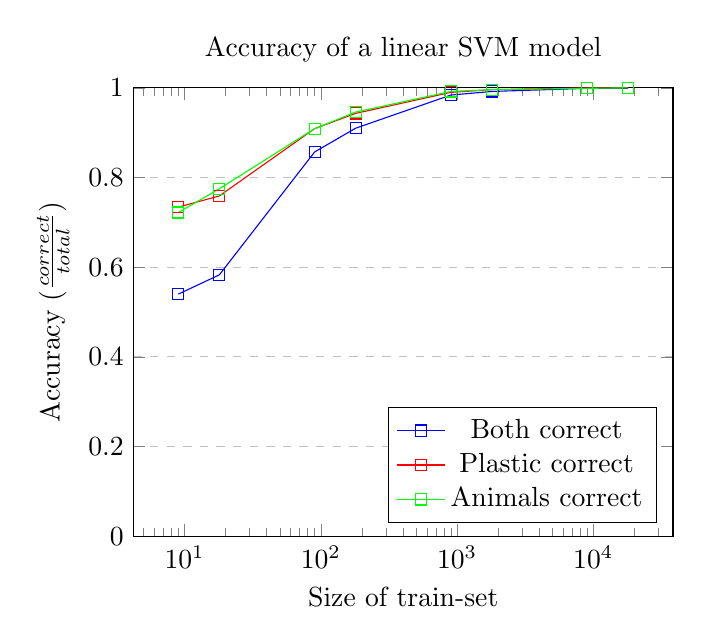
\begin{tikzpicture}
\begin{semilogxaxis}[
    title={Accuracy of a linear SVM model},
    xlabel={Size of train-set},
    ylabel={Accuracy ($\frac{correct}{total}$)},
    %xmin=0, xmax=18000,
    ymin=0, ymax=1,
    legend pos=south east,
    ymajorgrids=true,
    grid style=dashed,
]
\addplot[
    color=blue,
    mark=square,
    ]
    coordinates {
    %(14,0.571)(140,0.898)(1400,0.993)(14000,0.999)
     (9,0.540) (18,0.583) (90,0.857) (180,0.910) (900,0.984) (1800,0.992) (9000,0.999) (18000,0.999)
    };
    \addlegendentry{Both correct}
\addplot[
    color=red,
    mark=square,
    ]
    coordinates {
    (9,0.734) (18,0.759) (90,0.909) (180,0.943) (900,0.990) (1800,0.996) (9000,1.000) (18000,1.000)
    %(14,0.741)(140,0.947)(1400,0.996)(14000,1.000)
    };
    \addlegendentry{Plastic correct}
\addplot[
    color=green,
    mark=square,
    ]
    coordinates {
    (9,0.722) (18,0.775) (90,0.909) (180,0.946) (900,0.992) (1800,0.996) (9000,0.999) (18000,1.000)
    %(14,0.766)(140,0.924)(1400,0.997)(14000,0.999)
    };
    \addlegendentry{Animals correct}
\end{semilogxaxis}
\end{tikzpicture}
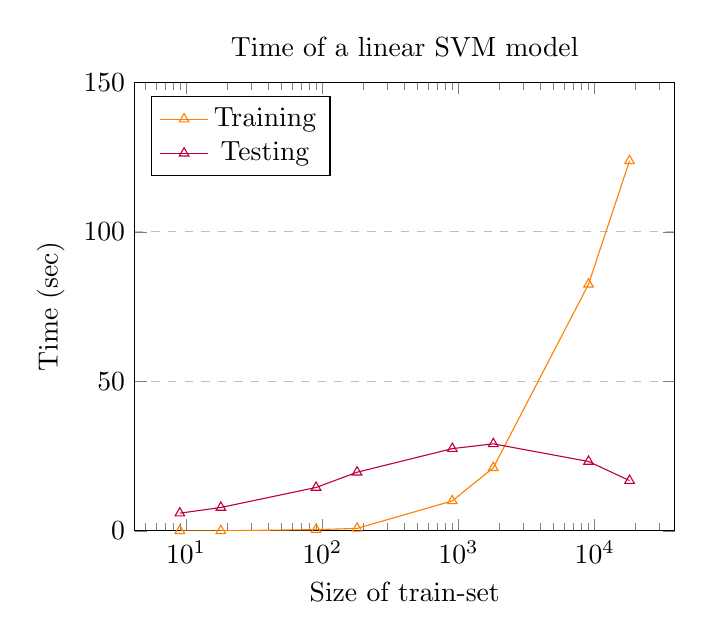
\begin{tikzpicture}
\begin{semilogxaxis}[
    title={Time of a linear SVM model},
    xlabel={Size of train-set},
    ylabel={Time (sec)},
    %xmin=0, xmax=18000,
    ymin=0, ymax=150,
    legend pos=north west,
    ymajorgrids=true,
    grid style=dashed,
    ]
\addplot[
    color=orange,
    mark=triangle,
    ]
    coordinates {
    (9,0.0) (18,0.0) (90,0.4) (180,0.8) (900,10.0) (1800,21.1) (9000,82.5) (18000,123.8)
    %(14,0.0)(140,0.2)(1400,5.6)(14000,74.6)
    };
    \addlegendentry{Training}
\addplot[
    color=purple,
    mark=triangle,
    ]
    coordinates {
    (9,5.9) (18,7.8) (90,14.5) (180,19.6) (900,27.5) (1800,29.1) (9000,23.2) (18000,16.8)
    %(14,0.6)(140,3.1)(1400,8.3)(14000,8.4)
    };
    \addlegendentry{Testing} 
\end{semilogxaxis}
\end{tikzpicture}
\end{minipage}
} \fi
\caption{Graph of time and accuracy of a linear SVM on different sizes data of the under water viewpoint. The test-data consisted of 4123 images. Large datasets show a high accuracy, however even small amounts of data show satisfying results.}
\label{fig:lin1}
\end{figure}

\begin{figure}%[h!tb]
\centering
\ifx\showfig\undefined
\centerline{
\begin{minipage}{1.3\textwidth}
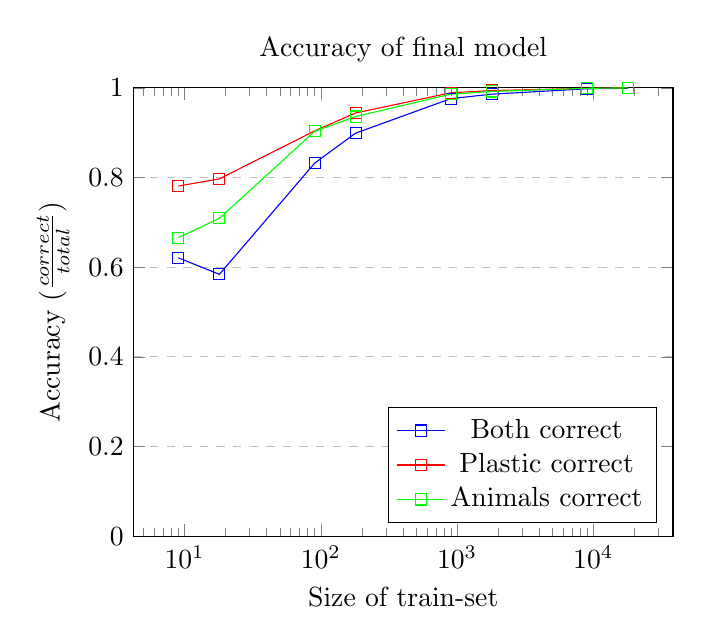
\begin{tikzpicture}
\begin{semilogxaxis}[
    title={Accuracy of final model},
    xlabel={Size of train-set},
    ylabel={Accuracy ($\frac{correct}{total}$)},
    %xmin=0, xmax=18000,
    ymin=0, ymax=1,
    legend pos=south east,
    ymajorgrids=true,
    grid style=dashed,
]
\addplot[
    color=blue,
    mark=square,
    ]
    coordinates {
    (9,0.621)(18,0.584)(90,0.832)(180,0.899)(900,0.976)(1800,0.986)(9000,0.998)(18000,0.999)
    };
    \addlegendentry{Both correct}
\addplot[
    color=red,
    mark=square,
    ]
    coordinates {
    (9,0.781)(18,0.797)(90,0.904)(180,0.944)(900,0.989)(1800,0.994)(9000,0.999)(18000,1.000)
    };
    \addlegendentry{Plastic correct}
\addplot[
    color=green,
    mark=square,
    ]
    coordinates {
    (9,0.666)(18,0.709)(90,0.903)(180,0.936)(900,0.986)(1800,0.992)(9000,0.999)(18000,1.000)
    };
    \addlegendentry{Animals correct}
\end{semilogxaxis}
\end{tikzpicture}
\hspace{.5cm}
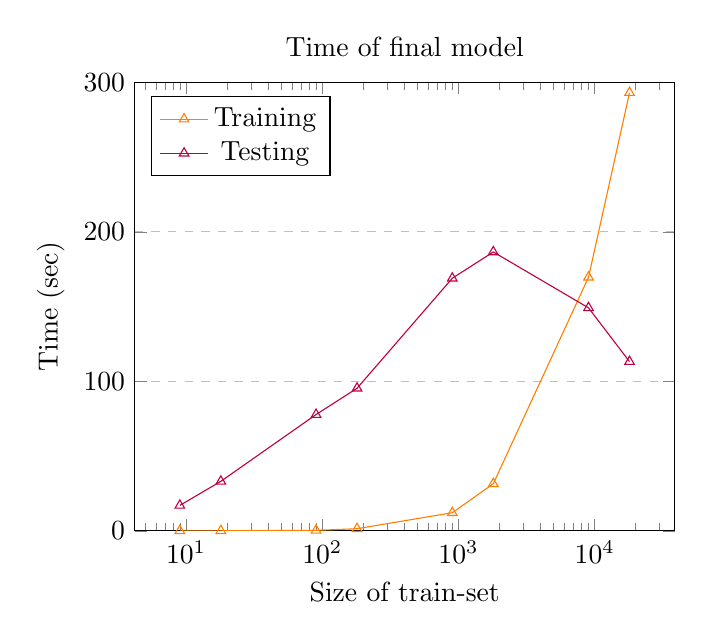
\begin{tikzpicture}
\begin{semilogxaxis}[
    title={Time of final model},
    xlabel={Size of train-set},
    ylabel={Time (sec)},
    %xmin=0, xmax=18000,
    ymin=0, ymax=300,
    legend pos=north west,
    ymajorgrids=true,
    grid style=dashed,
    ]
\addplot[
    color=orange,
    mark=triangle,
    ]
    coordinates {
    (9,0.0)(18,0.0)(90,0.3)(180,1.4)(900,12.1)(1800,31.5)(9000,169.7)(18000,293.2)
    };
    \addlegendentry{Training}
\addplot[
    color=purple,
    mark=triangle,
    ]
    coordinates {
    (9,17.0)(18,33.1)(90,77.8)(180,95.4)(900,169.0)(1800,186.6)(9000,149.2)(18000,113.2)
    };
    \addlegendentry{Testing} 
\end{semilogxaxis}
\end{tikzpicture}
\end{minipage}
} \fi
\caption{Graph of time and accuracy of a linear SVM on different sizes data of the under water viewpoint. The test-data consisted of 18583 images. The same trend as the graphs in figure \ref{fig:lin1} is seen.}
\label{fig:lin2}
\end{figure}

\subsection{Detecting the location of plastic}
\label{sec:Results-location}
As stated in section \ref{sec:Method-location}, the localisation of plastic within the image could not be evaluated truly.
However, several images were pulled through the pipeline and the results can be seen in figure \ref{fig:sub-matrix}.
The middle column in the figure shows the tested images.
The more red it shows in the figure on the right, the more confidence the program has in detecting plastic on that location in the image.
The images on the left represent the same with the greenness for locating animals.
Testing the localisation took a considerable amount of time, because a run through the pipeline could take up to $5$ seconds per sub-image.
Because these tests were conducted on a pyramid-segmentation of depth 4, a total amount of 341 images were run through the pipeline per test.

The results show that the confidence of detecting plastic or animals within the image does not always agree with what is shown in the original image.
However, because the lack of annotation, there is no manner in which these results can evaluated thoroughly.

\begin{figure}%[h!tb]
\centering
\ifx\showfig\undefined
\def\segwidth{.22\textwidth}
\begin{tabular}{ccc}

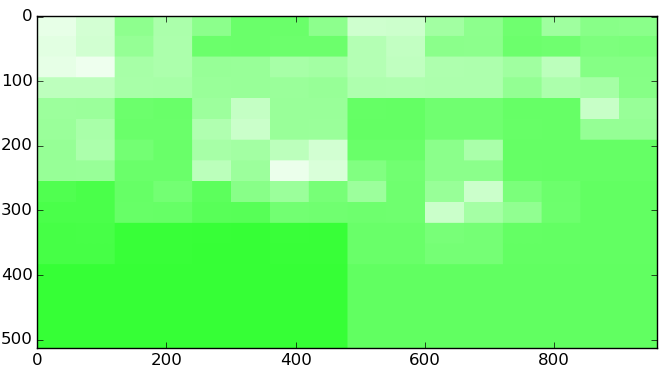
\includegraphics[keepaspectratio=true,width=\segwidth]{images/segment/6_01__animals__.png} &
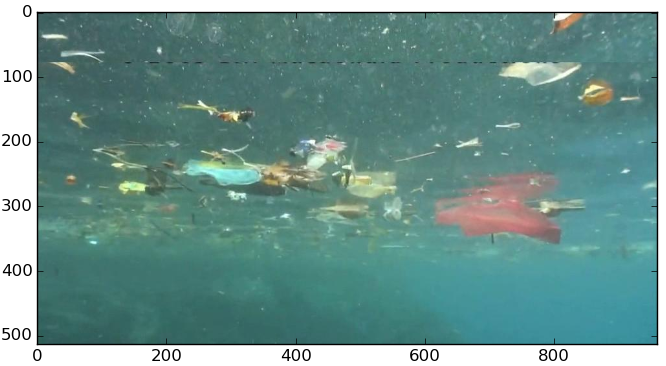
\includegraphics[keepaspectratio=true,width=\segwidth]{images/segment/6_01__image__.png} &
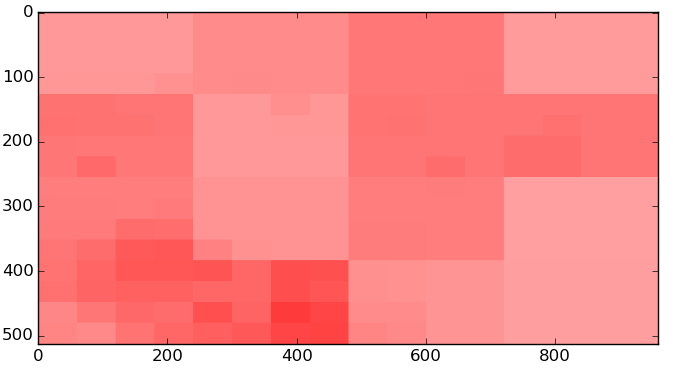
\includegraphics[keepaspectratio=true,width=\segwidth]{images/segment/6_01__plastic__.png} \\

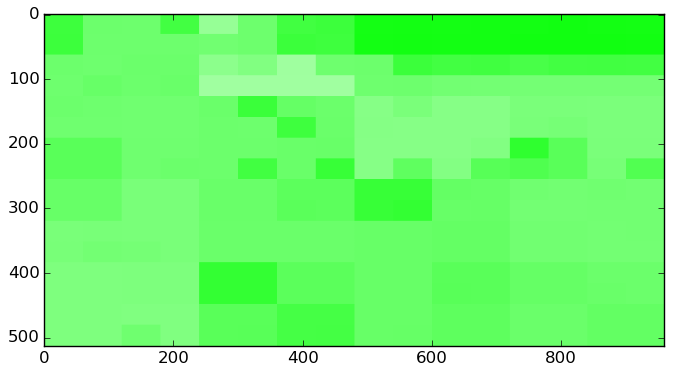
\includegraphics[keepaspectratio=true,width=\segwidth]{images/segment/31_11__animals__.png} &
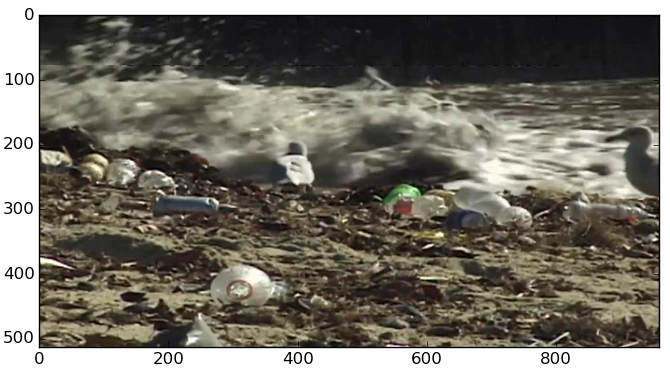
\includegraphics[keepaspectratio=true,width=\segwidth]{images/segment/31_11__image__.png} &
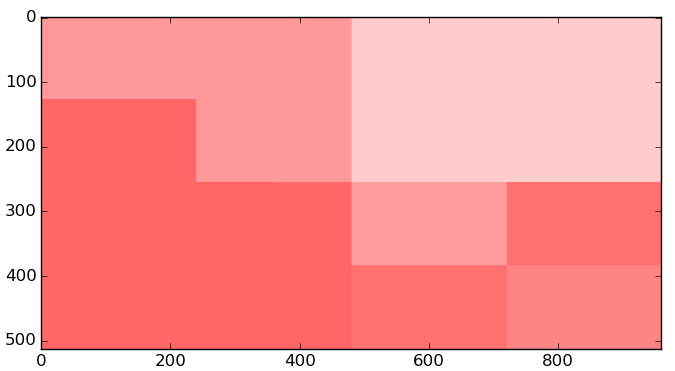
\includegraphics[keepaspectratio=true,width=\segwidth]{images/segment/31_11__plastic__.png} \\

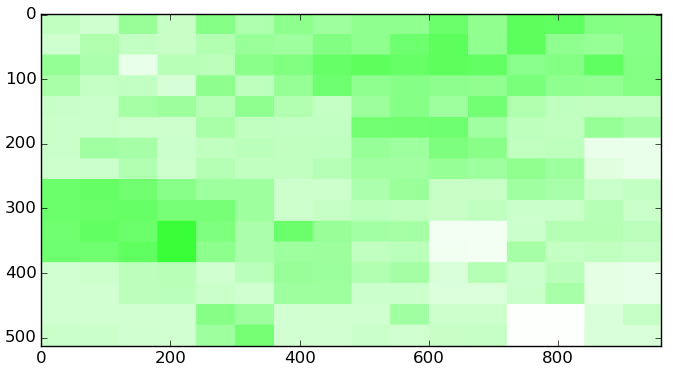
\includegraphics[keepaspectratio=true,width=\segwidth]{images/segment/253_01__animals__.png} &
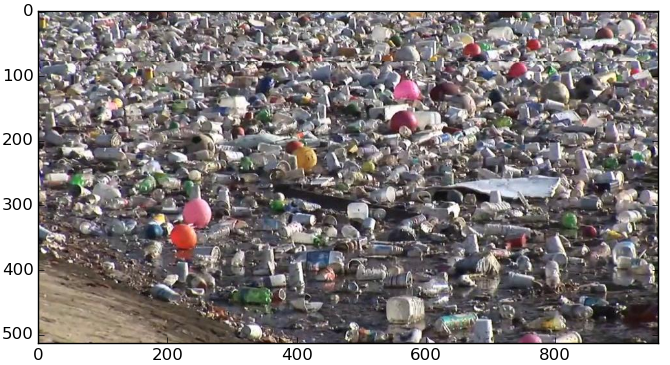
\includegraphics[keepaspectratio=true,width=\segwidth]{images/segment/253_01__image__.png} &
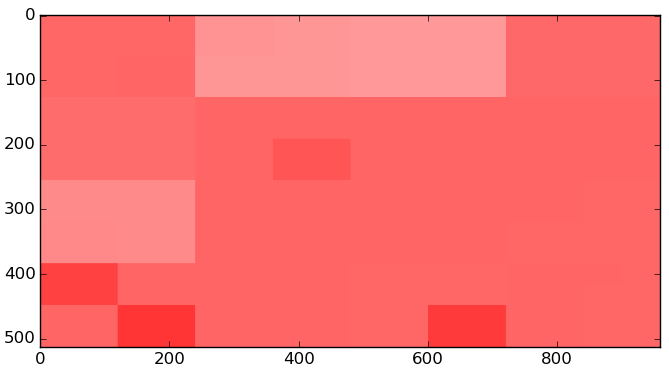
\includegraphics[keepaspectratio=true,width=\segwidth]{images/segment/253_01__plastic__.png} \\

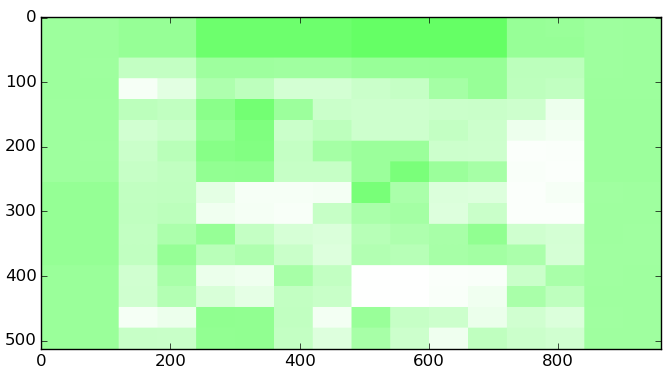
\includegraphics[keepaspectratio=true,width=\segwidth]{images/segment/299_00__animals__.png} &
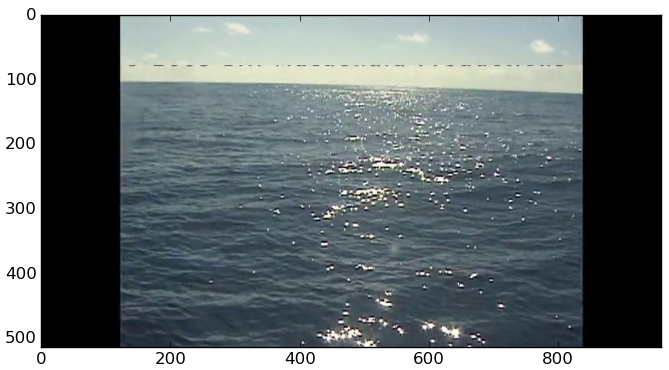
\includegraphics[keepaspectratio=true,width=\segwidth]{images/segment/299_00__image__.png} &
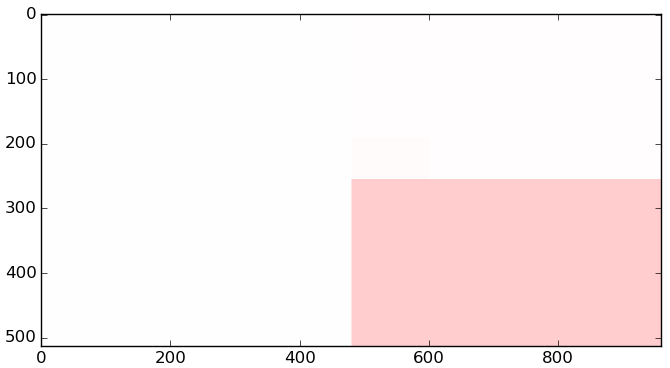
\includegraphics[keepaspectratio=true,width=\segwidth]{images/segment/299_00__plastic__.png} \\

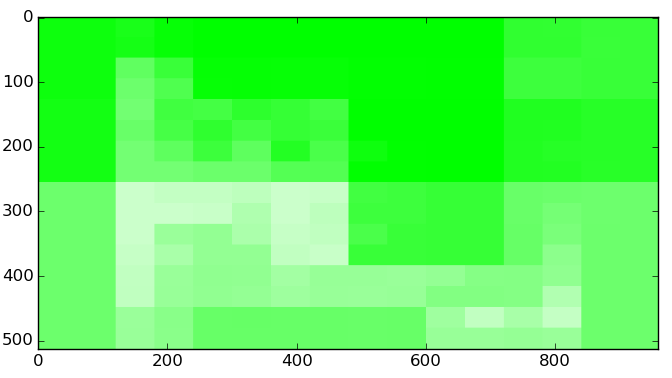
\includegraphics[keepaspectratio=true,width=\segwidth]{images/segment/401_10__animals__.png} &
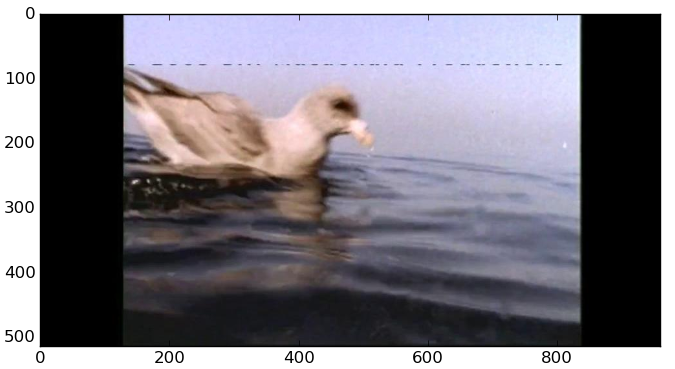
\includegraphics[keepaspectratio=true,width=\segwidth]{images/segment/401_10__image__.png} &
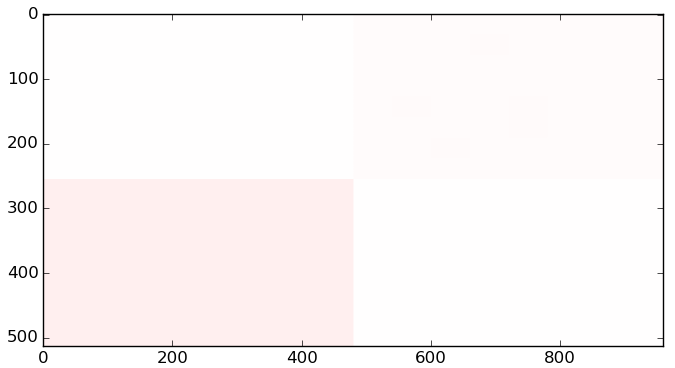
\includegraphics[keepaspectratio=true,width=\segwidth]{images/segment/401_10__plastic__.png} \\

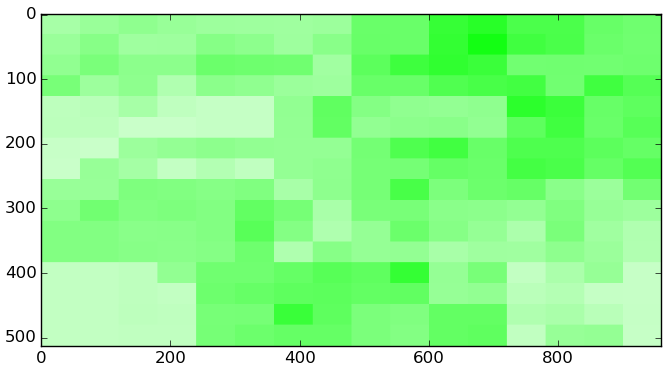
\includegraphics[keepaspectratio=true,width=\segwidth]{images/segment/701_11__animals__.png} &
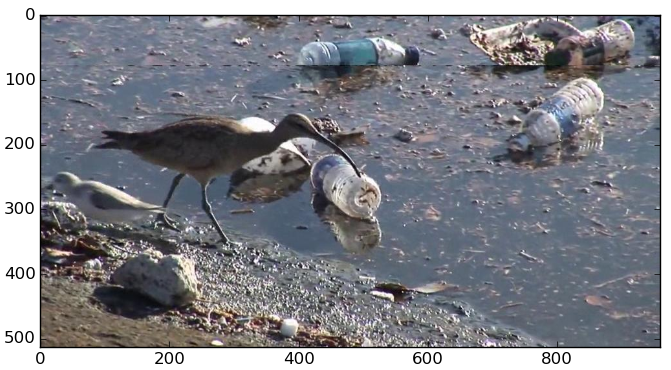
\includegraphics[keepaspectratio=true,width=\segwidth]{images/segment/701_11__image__.png} &
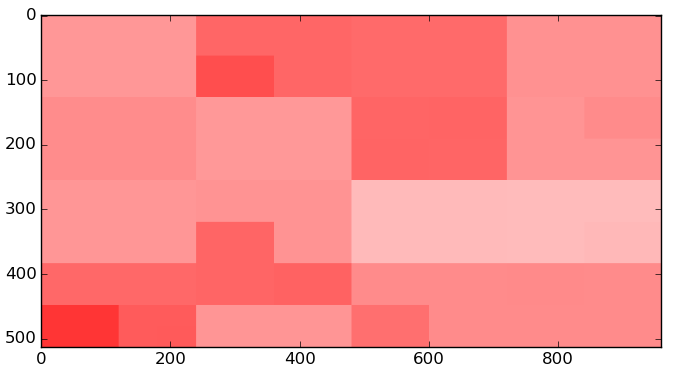
\includegraphics[keepaspectratio=true,width=\segwidth]{images/segment/701_11__plastic__.png} \\

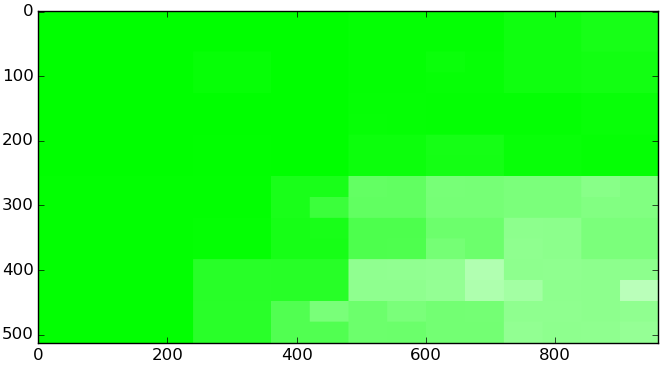
\includegraphics[keepaspectratio=true,width=\segwidth]{images/segment/2737_10__animals__.png} &
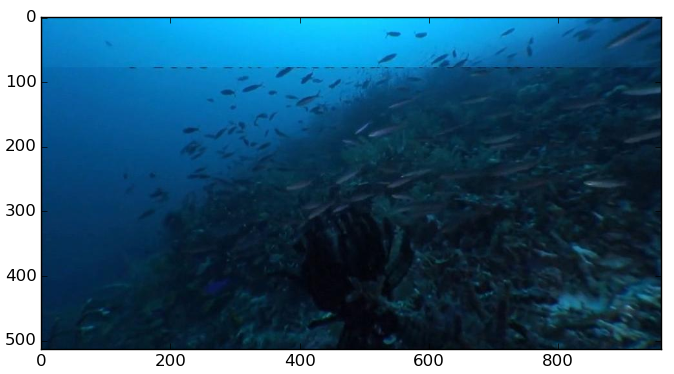
\includegraphics[keepaspectratio=true,width=\segwidth]{images/segment/2737_10__image__.png} &
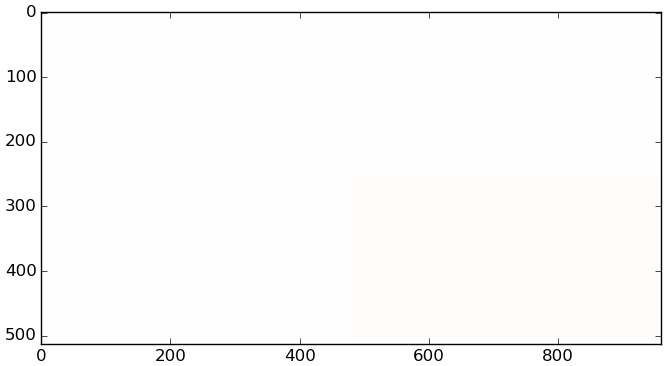
\includegraphics[keepaspectratio=true,width=\segwidth]{images/segment/2737_10__plastic__.png} \\

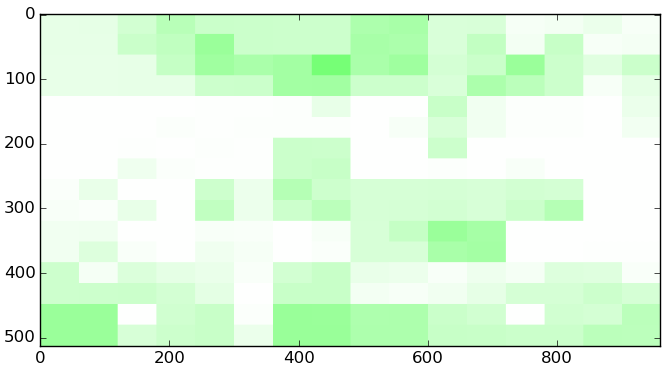
\includegraphics[keepaspectratio=true,width=\segwidth]{images/segment/4409_01__animals__.png} &
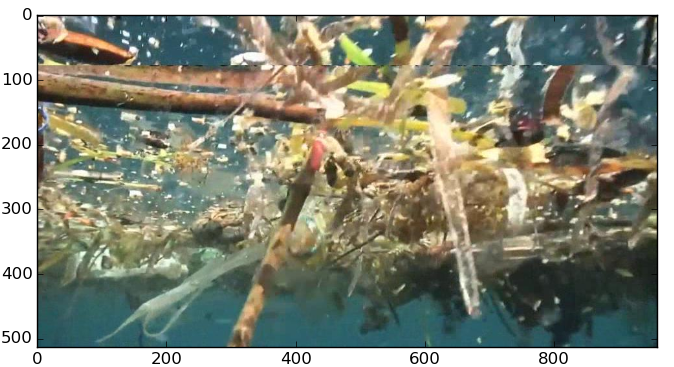
\includegraphics[keepaspectratio=true,width=\segwidth]{images/segment/4409_01__image__.png} &
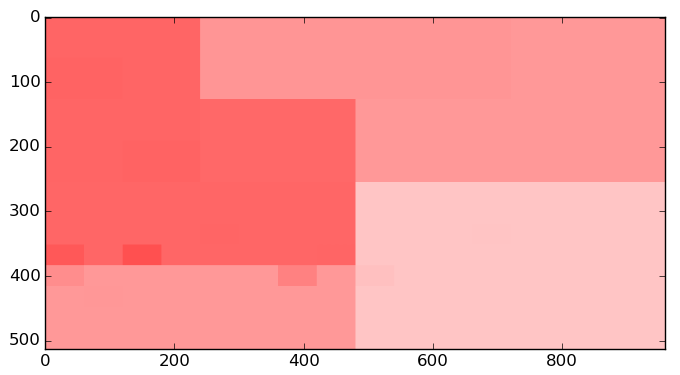
\includegraphics[keepaspectratio=true,width=\segwidth]{images/segment/4409_01__plastic__.png} \\

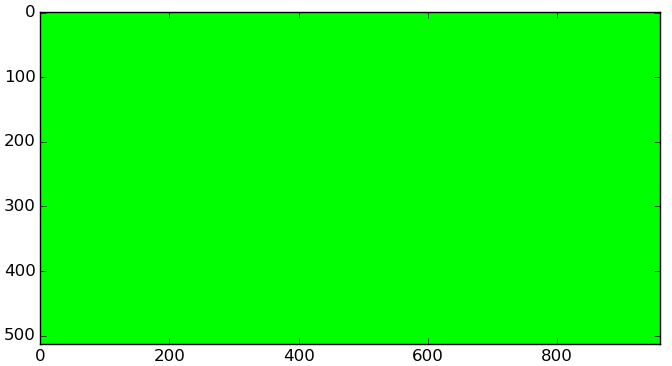
\includegraphics[keepaspectratio=true,width=\segwidth]{images/segment/5053_10__animals__.png} &
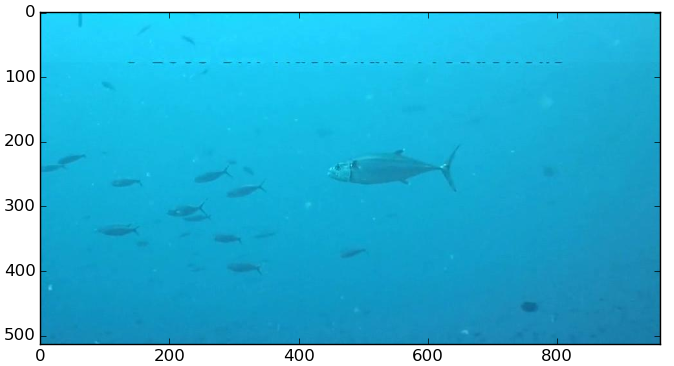
\includegraphics[keepaspectratio=true,width=\segwidth]{images/segment/5053_10__image__.png} &
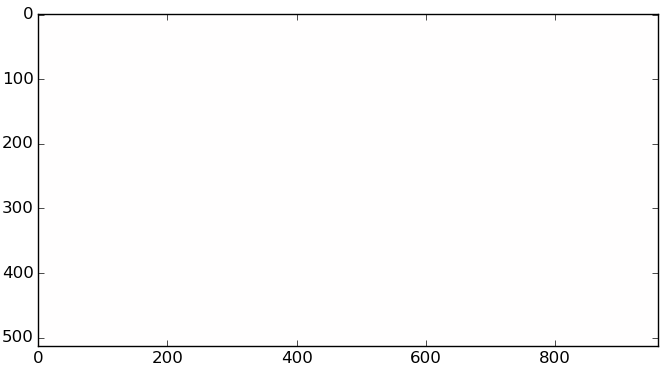
\includegraphics[keepaspectratio=true,width=\segwidth]{images/segment/5053_10__plastic__.png} \\

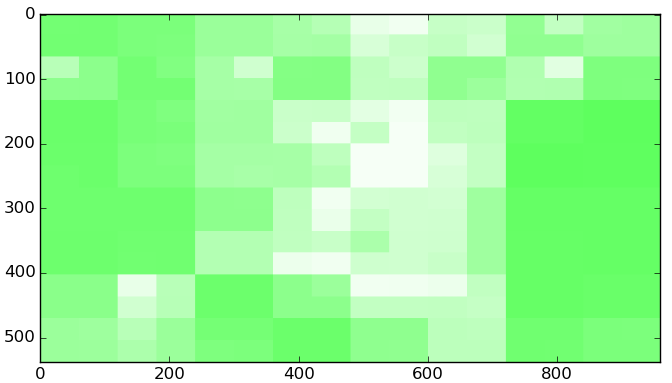
\includegraphics[keepaspectratio=true,width=\segwidth]{images/segment/20607_01__animals__.png} &
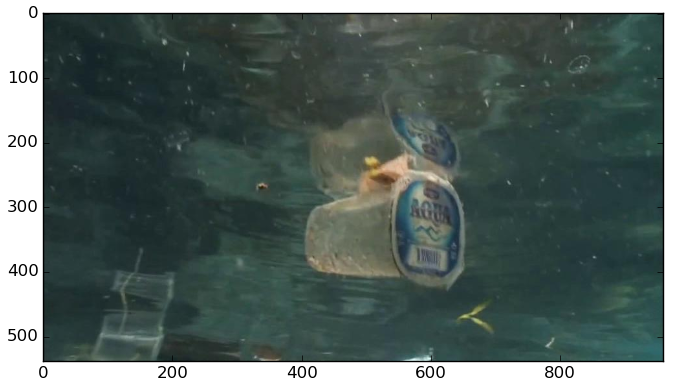
\includegraphics[keepaspectratio=true,width=\segwidth]{images/segment/20607_01__image__.png} &
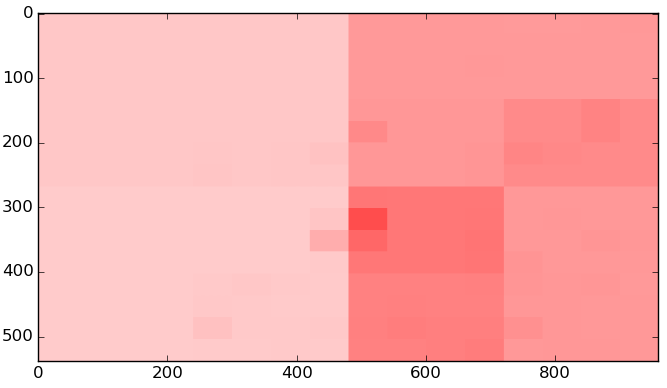
\includegraphics[keepaspectratio=true,width=\segwidth]{images/segment/20607_01__plastic__.png}
	\end{tabular}
\fi
\captionsetup{width=.8\textwidth}
\caption{Example of outcome of running an image through the segmented image pipeline. Green locates the animals and red the plastic}
\label{fig:sub-matrix}
\end{figure}